\section{Trabalhos Relacionados}
\label{sec:trabalhosRelacionados}

O artigo \cite{designImplementationSIG} possui similaridades com a nossa solução de Smart IoT Gateway, ele apresenta um software Smart Iot Gateway flexível que pode ser configurado para se adaptar a diferentes requisitos, e com isso reduzir o ciclo de desenvolvimento, custos. O Smart IoT Gateway tem como responsabilidade controlar os diferentes protocolos de comunicação, identificar os tipos de dispositivos e possíveis tratamentos de mensagens. Além disso, o gateway possui algumas interfaces externas unificadas, capazes de se adaptar à diferentes necessidades, onde os usuários podem desenvolver cartões apropriados de acordo com diferentes aplicativos. Como ethernet (RJ45), USB, som e interfaces de vídeo, ver Figura~\ref{fig:arquiteturaDesignImpelementationSmartIoTGateway}.

\begin{figure}[h!]
	\begin{center}
		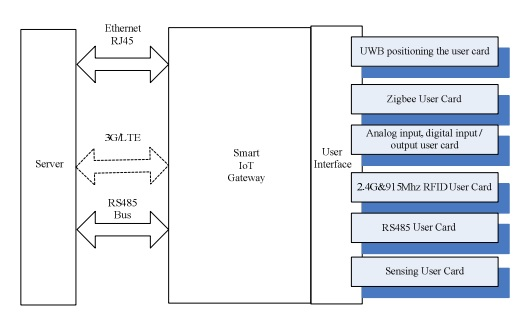
\includegraphics[width=0.8\textwidth]{./img/arquiteturaDesignImpelementationSmartIoTGateway}
		\caption{Arquitetura do Smart IoT Gateway.}
		\label{fig:arquiteturaDesignImpelementationSmartIoTGateway}
	\end{center}
\end{figure}


 